
\chapter{Projeto da Lógica de Negócio}
\label{sec-logica-negocio}
\vspace{-1cm}

Este capítulo apresenta o projeto da camada de Negócio dos três subsistemas do Happy Paws: Gestão de Perfis, Serviços e Suporte (Figura~\ref{figura-arquitetura}).

Para organizar a lógica de negócio foi usado o padrão Camada de Serviço (\textit{Service Layer})~\cite{fowler:book02}. Com ele, a camada de Negócio de cada subsistema é dividida em dois componentes:

\begin{itemize}
	\item \textbf{Componente de Domínio do Problema (CDP):} tem as classes do domínio (Tutor, Cachorro, Agendamento, Passeio, Chamado etc.), com seus atributos e os métodos que tratam das regras de cada objeto, como verificar se um Passeio pode ser iniciado ou se um Pagamento já foi pago;
	\item \textbf{Componente de Gerência de Tarefas (CGT):} tem as classes de aplicação (prefixo \texttt{Apl}), que realizam as histórias de usuário. Elas recebem as requisições da camada de Apresentação, buscam os objetos nos repositórios da camada de Acesso a Dados, chamam os métodos do CDP e salvam o resultado. No Happy Paws, cada classe de aplicação é implementada como um módulo de \emph{Server Actions} do Next.js.
\end{itemize}

Esse padrão foi escolhido por três motivos: Primeiro, as \emph{Server Actions} já funcionam como pontos de entrada para cada funcionalidade, o que corresponde diretamente às operações do CGT. Segundo, várias histórias envolvem muitas classes ao mesmo tempo, inclusive de subsistemas diferentes: agendar um passeio, por exemplo, envolve Tutor, Cachorro, Passeador, Agendamento e Pagamento, e essa coordenação fica mais clara em uma classe de aplicação do que espalhada pelas classes de domínio. Terceiro, a relação direta entre classes de aplicação e histórias de usuário facilita a manutenção: quando uma história muda, sabe-se qual classe alterar. Para não cair em um modelo de domínio anêmico, as regras que dizem respeito a um único objeto continuam como métodos das classes do CDP, e o CGT apenas coordena esses objetos.

A Tabela~\ref{tabela-componentes-negocio} resume os componentes da camada de Negócio de cada subsistema.

\begin{footnotesize}
\begin{longtable}{|p{2.6cm}|p{5.4cm}|p{5.4cm}|}
	\caption{Componentes da camada de Negócio por subsistema.}
	\label{tabela-componentes-negocio}\\\hline

	\rowcolor{lightgray}
	\textbf{Subsistema} & \textbf{CDP} & \textbf{CGT} \\\hline
	\endfirsthead
	\hline
	\rowcolor{lightgray}
	\textbf{Subsistema} & \textbf{CDP} & \textbf{CGT} \\\hline
	\endhead

	Gestão de Perfis & \texttt{Usuario}, \texttt{Tutor}, \texttt{Passeador}, \texttt{Atendente}, \texttt{Endereco}, \texttt{Cachorro}, \texttt{ConviteCompartilhamento}, \texttt{Validacao}, \texttt{Documento} & \texttt{AplCadastroUsuario}, \texttt{AplCadastroCachorro}, \texttt{AplCompartilhamentoPerfil}, \texttt{AplValidacaoPasseador} \\\hline

	Serviços & \texttt{Agendamento}, \texttt{Passeio}, \texttt{RegistroPasseio}, \texttt{Foto}, \texttt{Pagamento}, \texttt{Avaliacao}, \texttt{Conquista}, \texttt{ConquistaObtida} & \texttt{AplBuscaPasseadores}, \texttt{AplAgendamento}, \texttt{AplPagamento}, \texttt{AplExecucaoPasseio}, \texttt{AplAvaliacao}, \texttt{AplConquistas} \\\hline

	Suporte & \texttt{Chamado}, \texttt{RespostaChamado} & \texttt{AplChamado}, \texttt{AplAtendimento} \\\hline
\end{longtable}
\end{footnotesize}



\section{Dependências entre os Subsistemas}
\label{sec-logica-dependencias}

Os subsistemas não são independentes: classes de um subsistema fazem referência a classes de outro. A Figura~\ref{figura-ln-pacotes} mostra o diagrama de pacotes da camada de Negócio com essas dependências.

\begin{figure}[h!]
	\centering
	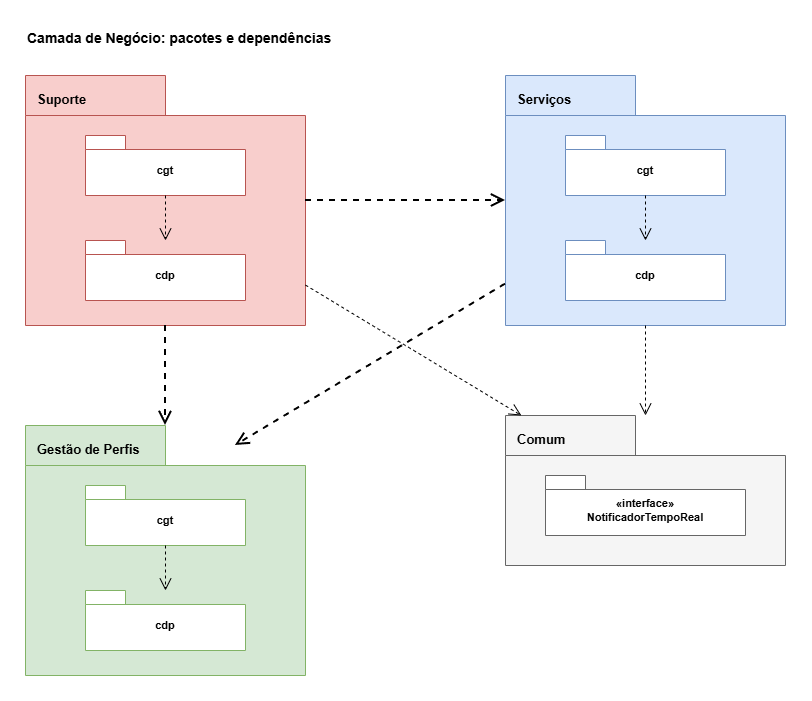
\includegraphics[width=0.85\textwidth]{figuras/ln-pacotes.png}
	\caption{Diagrama de pacotes da camada de Negócio, com as dependências entre os subsistemas.}
	\label{figura-ln-pacotes}
\end{figure}

\begin{itemize}
	\item \textbf{Serviços depende de Gestão de Perfis:} um \texttt{Agendamento} referencia o \texttt{Tutor} que o solicitou, o \texttt{Passeador} que vai realizá-lo e os \texttt{Cachorro}s que vão passear; uma \texttt{ConquistaObtida} referencia o \texttt{Cachorro} que a recebeu. A busca de passeadores também usa o \texttt{Endereco} e as especialidades do \texttt{Passeador};
	\item \textbf{Suporte depende de Gestão de Perfis:} um \texttt{Chamado} é aberto por um \texttt{Usuario} (Tutor ou Passeador) e cada \texttt{RespostaChamado} é escrita por um \texttt{Atendente};
	\item \textbf{Suporte depende de Serviços:} um \texttt{Chamado} pode estar ligado a um \texttt{Passeio}, quando o problema relatado aconteceu durante um passeio (por exemplo, um chamado de emergência).
\end{itemize}

As dependências seguem sempre o mesmo sentido (Suporte $\rightarrow$ Serviços $\rightarrow$ Gestão de Perfis) e não há ciclos. Gestão de Perfis não depende de nenhum outro subsistema e, por isso, pode ser implementado e testado primeiro. As associações entre classes de subsistemas diferentes são navegáveis apenas nesse sentido: um \texttt{Agendamento} conhece o seu \texttt{Tutor}, mas a classe \texttt{Tutor} não guarda a lista de agendamentos (essa consulta é feita pelo \texttt{AgendamentoRepository}).



\section{Decisões de Projeto Comuns aos Subsistemas}
\label{sec-logica-decisoes}

Para passar dos diagramas de classes de análise para os diagramas de classes de projeto, foram tomadas as decisões abaixo, que valem para os três subsistemas:

\begin{itemize}
	\item \textbf{Tipos de dados:} os atributos receberam tipos do TypeScript (\texttt{string}, \texttt{number}, \texttt{boolean} e \texttt{Date}). Identificadores são \texttt{string} no formato UUID. Valores em dinheiro são guardados como \texttt{number} inteiro em centavos (por exemplo, \texttt{valorCentavos}), para evitar erros de arredondamento. Atributos opcionais são indicados com multiplicidade \texttt{[0..1]} e implementados como \texttt{tipo | null};

	\item \textbf{Tipos enumerados:} atributos que só podem assumir alguns valores viraram tipos enumerados (Tabela~\ref{tabela-enumerados}). Isso permite que a camada de Apresentação mostre esses valores em listas de seleção, em vez de campos de texto livre, reduzindo erros de digitação e o número de ações do usuário. No banco, eles são mapeados para \texttt{pgEnum} do Drizzle ORM;

	\item \textbf{Navegabilidade:} as associações passaram a ter sentido de navegação, escolhido a partir das consultas mais frequentes. Por exemplo, \texttt{Passeio} navega para os seus \texttt{RegistroPasseio} (para desenhar o trajeto), mas \texttt{RegistroPasseio} não navega de volta. Entre subsistemas, a navegação segue o sentido das dependências da Seção~\ref{sec-logica-dependencias};

	\item \textbf{Visibilidade e métodos:} todos os atributos são privados. Os métodos de acesso (\texttt{get}/\texttt{set}), construtores e destrutores existem, mas não aparecem nos diagramas. Só são mostrados os métodos que não podem ser deduzidos dos atributos, isto é, os que implementam regras de negócio;

	\item \textbf{Ajuste de hierarquia:} Tutor, Passeador e Atendente têm em comum nome, CPF, e-mail, senha e telefone. Foi criada a superclasse abstrata \texttt{Usuario} com esses dados e com o método de autenticação. Isso também permite que um \texttt{Chamado} seja aberto por qualquer usuário;

	\item \textbf{Eliminação de classe associativa:} a associação entre \texttt{Cachorro} e \texttt{Conquista} guarda a data em que a conquista foi obtida. Como o TypeScript não tem um recurso para classes associativas, ela foi substituída pela classe \texttt{ConquistaObtida}, ligada a \texttt{Cachorro} e a \texttt{Conquista};

	\item \textbf{Segurança:} a senha é guardada apenas como \textit{hash} (\texttt{senhaHash}); \texttt{Pagamento} guarda só o identificador da transação no provedor de pagamento e os quatro últimos dígitos do cartão; e toda operação do CGT recebe o usuário autenticado da sessão e verifica se ele tem permissão sobre os objetos envolvidos (por exemplo, só o tutor e o passeador de um passeio podem ver o seu trajeto), conforme o \ref{rnf-seguranca-dados}.
\end{itemize}

\begin{footnotesize}
\begin{longtable}{|p{3.2cm}|p{5.8cm}|p{4.4cm}|}
	\caption{Tipos enumerados da camada de Negócio.}
	\label{tabela-enumerados}\\\hline

	\rowcolor{lightgray}
	\textbf{Tipo Enumerado} & \textbf{Valores} & \textbf{Usado em} \\\hline
	\endfirsthead
	\hline
	\rowcolor{lightgray}
	\textbf{Tipo Enumerado} & \textbf{Valores} & \textbf{Usado em} \\\hline
	\endhead

	\texttt{Porte} & Pequeno, Médio, Grande & \texttt{Cachorro} \\\hline
	\texttt{Especialidade} & Filhotes, Idosos, Grande Porte, Cães Reativos & \texttt{Passeador} \\\hline
	\texttt{TipoDocumento} & RG, CNH, Selfie, CPF & \texttt{Documento} \\\hline
	\texttt{StatusValidacao} & Em Análise, Validado, Reprovado & \texttt{Validacao} \\\hline
	\texttt{StatusConvite} & Pendente, Ativo, Recusado & \texttt{ConviteCompartilhamento} \\\hline
	\texttt{TipoAgendamento} & Avulso, Recorrente & \texttt{Agendamento} \\\hline
	\texttt{DiaSemana} & Domingo a Sábado & \texttt{Agendamento} (passeios fixos) \\\hline
	\texttt{StatusAgendamento} & Pendente, Confirmado, Cancelado, Concluído & \texttt{Agendamento} \\\hline
	\texttt{StatusPasseio} & Agendado, Iniciado, Concluído, Cancelado & \texttt{Passeio} \\\hline
	\texttt{TipoRegistro} & Posição, Alerta de Incidente & \texttt{RegistroPasseio} \\\hline
	\texttt{MetodoPagamento} & Cartão de Crédito, Pix & \texttt{Pagamento} \\\hline
	\texttt{StatusPagamento} & Processando, Pago, Recusado, Estornado & \texttt{Pagamento} \\\hline
	\texttt{CriterioConquista} & Quantidade de Passeios, Distância Percorrida & \texttt{Conquista} \\\hline
	\texttt{TipoChamado} & Financeiro, Emergência, Técnico, Denúncia, Outros & \texttt{Chamado} \\\hline
	\texttt{StatusChamado} & Em análise, Em atendimento, Resolvido & \texttt{Chamado} \\\hline
\end{longtable}
\end{footnotesize}



\section{Subsistema Gestão de Perfis}
\label{sec-logica-perfis}

O subsistema Gestão de Perfis cuida do cadastro de tutores, cães e passeadores, da validação de identidade dos passeadores e do compartilhamento de perfis de cães entre tutores (US01 a US06).


\subsection{Componente de Domínio do Problema}
\label{sec-logica-perfis-cdp}

A Figura~\ref{figura-ln-perfis-cdp} mostra o diagrama de classes do CDP do subsistema Gestão de Perfis.

\begin{figure}[h!]
	\centering
	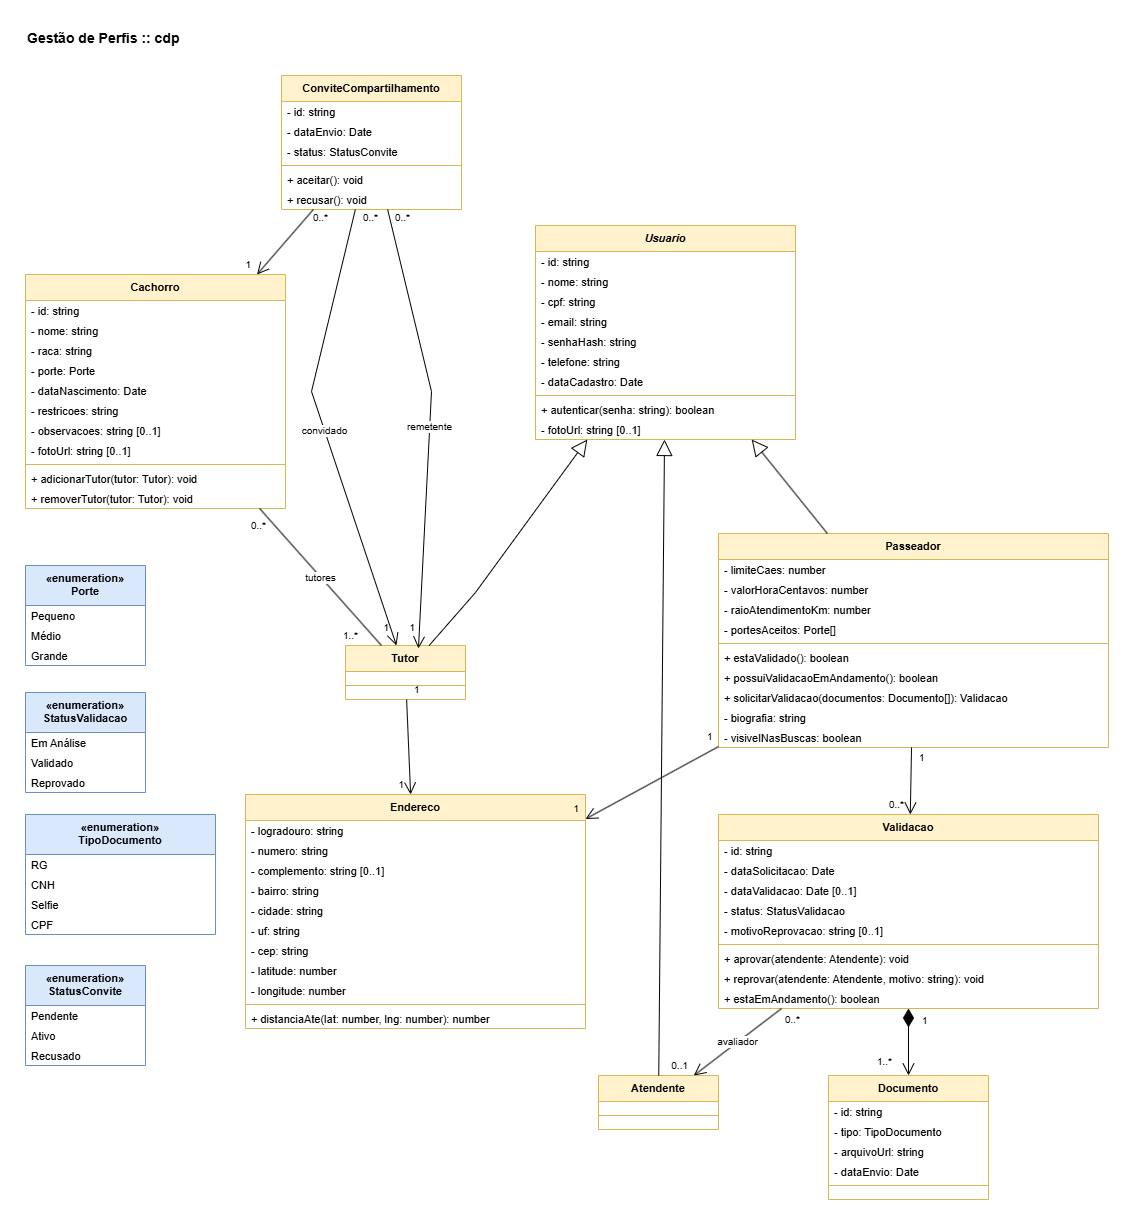
\includegraphics[width=\textwidth]{figuras/ln-perfis-cdp.png}
	\caption{Diagrama de classes do CDP do subsistema Gestão de Perfis.}
	\label{figura-ln-perfis-cdp}
\end{figure}

As principais classes e métodos são:

\begin{itemize}
	\item \texttt{Usuario} (abstrata): superclasse de \texttt{Tutor}, \texttt{Passeador} e \texttt{Atendente}, com \texttt{id}, \texttt{nome}, \texttt{cpf}, \texttt{email}, \texttt{senhaHash}, \texttt{telefone} e \texttt{dataCadastro}. O método \texttt{autenticar(senha)} compara a senha informada com o \textit{hash} guardado;

	\item \texttt{Passeador}: tem \texttt{limiteCaes}, \texttt{valorHoraCentavos}, \texttt{raioAtendimentoKm} e uma lista de \texttt{Especialidade}. O método \texttt{estaValidado()} indica se o passeador já teve uma validação aprovada (só passeadores validados aparecem na busca); \texttt{possuiValidacaoEmAndamento()} e \texttt{solicitarValidacao(documentos)} garantem que o passeador não tenha mais de uma Validação ao mesmo tempo (RI-4);

	\item \texttt{Endereco}: além dos dados do endereço, guarda \texttt{latitude} e \texttt{longitude}. O método \texttt{distanciaAte(lat, lng)} é usado na busca de passeadores por geolocalização;

	\item \texttt{Cachorro}: tem \texttt{nome}, \texttt{raca}, \texttt{porte}, \texttt{dataNascimento}, \texttt{observacoes} e \texttt{fotoUrl}, e uma associação com um ou mais \texttt{Tutor}es, navegável nos dois sentidos, pois as consultas ``cães de um tutor'' e ``tutores de um cão'' são frequentes. O método \texttt{removerTutor(tutor)} impede a remoção do último tutor, garantindo a RI-3;

	\item \texttt{ConviteCompartilhamento}: classe criada para representar o convite da US05. Liga o cão, o tutor que convida e o tutor convidado, e tem os métodos \texttt{aceitar()}, que adiciona o convidado como tutor do cão, e \texttt{recusar()};

	\item \texttt{Validacao} e \texttt{Documento}: uma Validação é composta por um ou mais Documentos enviados pelo passeador. Os métodos \texttt{aprovar(atendente)} e \texttt{reprovar(atendente, motivo)} registram o atendente responsável e a data da validação, conferindo se a data de envio de todos os documentos é anterior ou igual a ela (RI-5).
\end{itemize}

As regras RI-1 e RI-2 (CPF e e-mail únicos) dependem de outros objetos já cadastrados e, por isso, não ficam em uma classe do CDP: elas são verificadas pela classe de aplicação \texttt{AplCadastroUsuario}, que consulta os repositórios antes de salvar.


\subsection{Componente de Gerência de Tarefas}
\label{sec-logica-perfis-cgt}

A Figura~\ref{figura-ln-perfis-cgt} mostra as classes do CGT do subsistema e a Tabela~\ref{tabela-cgt-perfis} descreve suas operações.

\begin{figure}[h!]
	\centering
	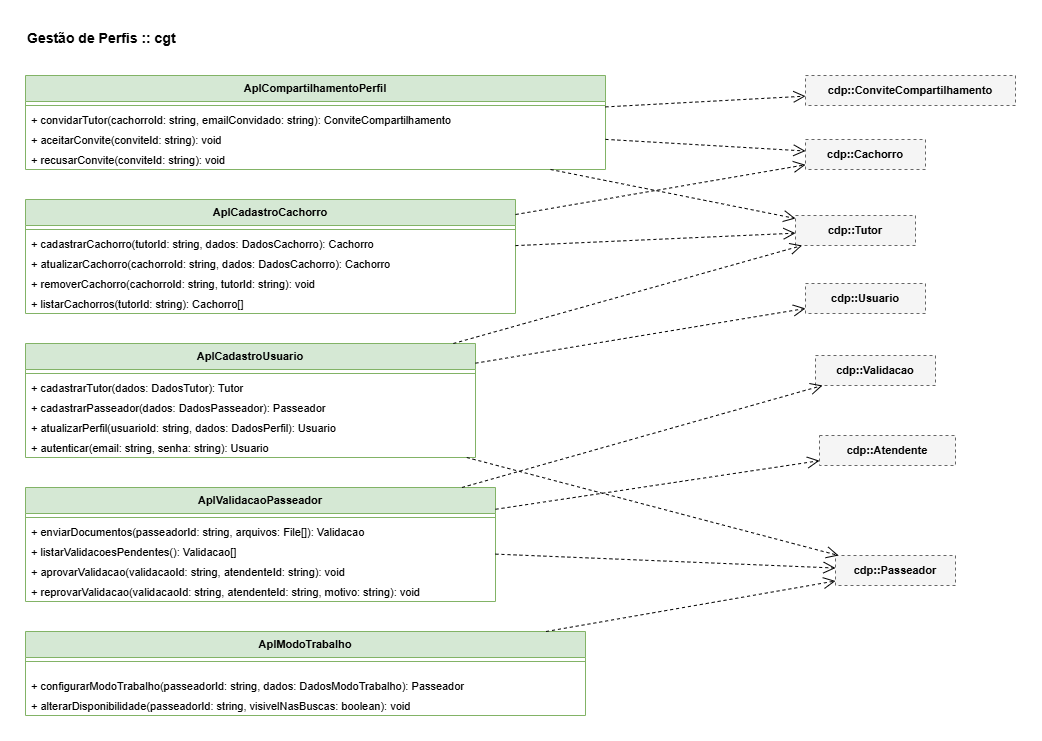
\includegraphics[width=\textwidth]{figuras/ln-perfis-cgt.png}
	\caption{Diagrama de classes do CGT do subsistema Gestão de Perfis.}
	\label{figura-ln-perfis-cgt}
\end{figure}

\begin{footnotesize}
\begin{longtable}{|p{3.4cm}|p{7.6cm}|p{2.4cm}|}
	\caption{Operações do CGT do subsistema Gestão de Perfis.}
	\label{tabela-cgt-perfis}\\\hline

	\rowcolor{lightgray}
	\textbf{Classe} & \textbf{Operações} & \textbf{Regras} \\\hline
	\endfirsthead
	\hline
	\rowcolor{lightgray}
	\textbf{Classe} & \textbf{Operações} & \textbf{Regras} \\\hline
	\endhead

	\texttt{AplCadastroUsuario} & \texttt{cadastrarTutor(dados)}: cadastra um tutor e seu endereço. \newline
	\texttt{cadastrarPasseador(dados)}: cadastra um passeador, com limite de cães e especialidades. \newline
	\texttt{atualizarPerfil(usuarioId, dados)}: altera os dados do perfil. \newline
	\texttt{autenticar(email, senha)}: faz o \textit{login} do usuário. & RI-1, RI-2 \\\hline

	\texttt{AplCadastroCachorro} & \texttt{cadastrarCachorro(tutorId, dados)}: cadastra um cão ligado ao tutor. \newline
	\texttt{atualizarCachorro(cachorroId, dados)}: altera os dados do cão. \newline
	\texttt{removerCachorro(cachorroId, tutorId)}: remove o cão ou desvincula o tutor. \newline
	\texttt{listarCachorros(tutorId)}: lista os cães do tutor. & RI-3 \\\hline

	\texttt{AplCompartilhamentoPerfil} & \texttt{convidarTutor(cachorroId, emailConvidado)}: cria um convite de compartilhamento. \newline
	\texttt{aceitarConvite(conviteId)}: o convidado passa a ser tutor do cão. \newline
	\texttt{recusarConvite(conviteId)}: encerra o convite. & US05 \\\hline

	\texttt{AplValidacaoPasseador} & \texttt{enviarDocumentos(passeadorId, arquivos)}: envia os documentos e abre uma validação. \newline
	\texttt{listarValidacoesPendentes()}: lista as validações para o Atendente. \newline
	\texttt{aprovarValidacao(validacaoId)}: aprova a validação. \newline
	\texttt{reprovarValidacao(validacaoId, motivo)}: reprova a validação, informando o motivo. & RI-4, RI-5 \\\hline
\end{longtable}
\end{footnotesize}



\section{Subsistema Serviços}
\label{sec-logica-servicos}

O subsistema Serviços cuida da busca por passeadores, do agendamento de passeios (avulsos ou fixos), da execução do passeio em tempo real (GPS, alertas e fotos), do pagamento, da avaliação e das conquistas do pet (US07 a US15).


\subsection{Componente de Domínio do Problema}
\label{sec-logica-servicos-cdp}

A Figura~\ref{figura-ln-servicos-cdp} mostra o diagrama de classes do CDP do subsistema Serviços. As classes \texttt{Tutor}, \texttt{Passeador} e \texttt{Cachorro} aparecem no diagrama como classes do pacote de Gestão de Perfis.

\begin{figure}[h!]
	\centering
	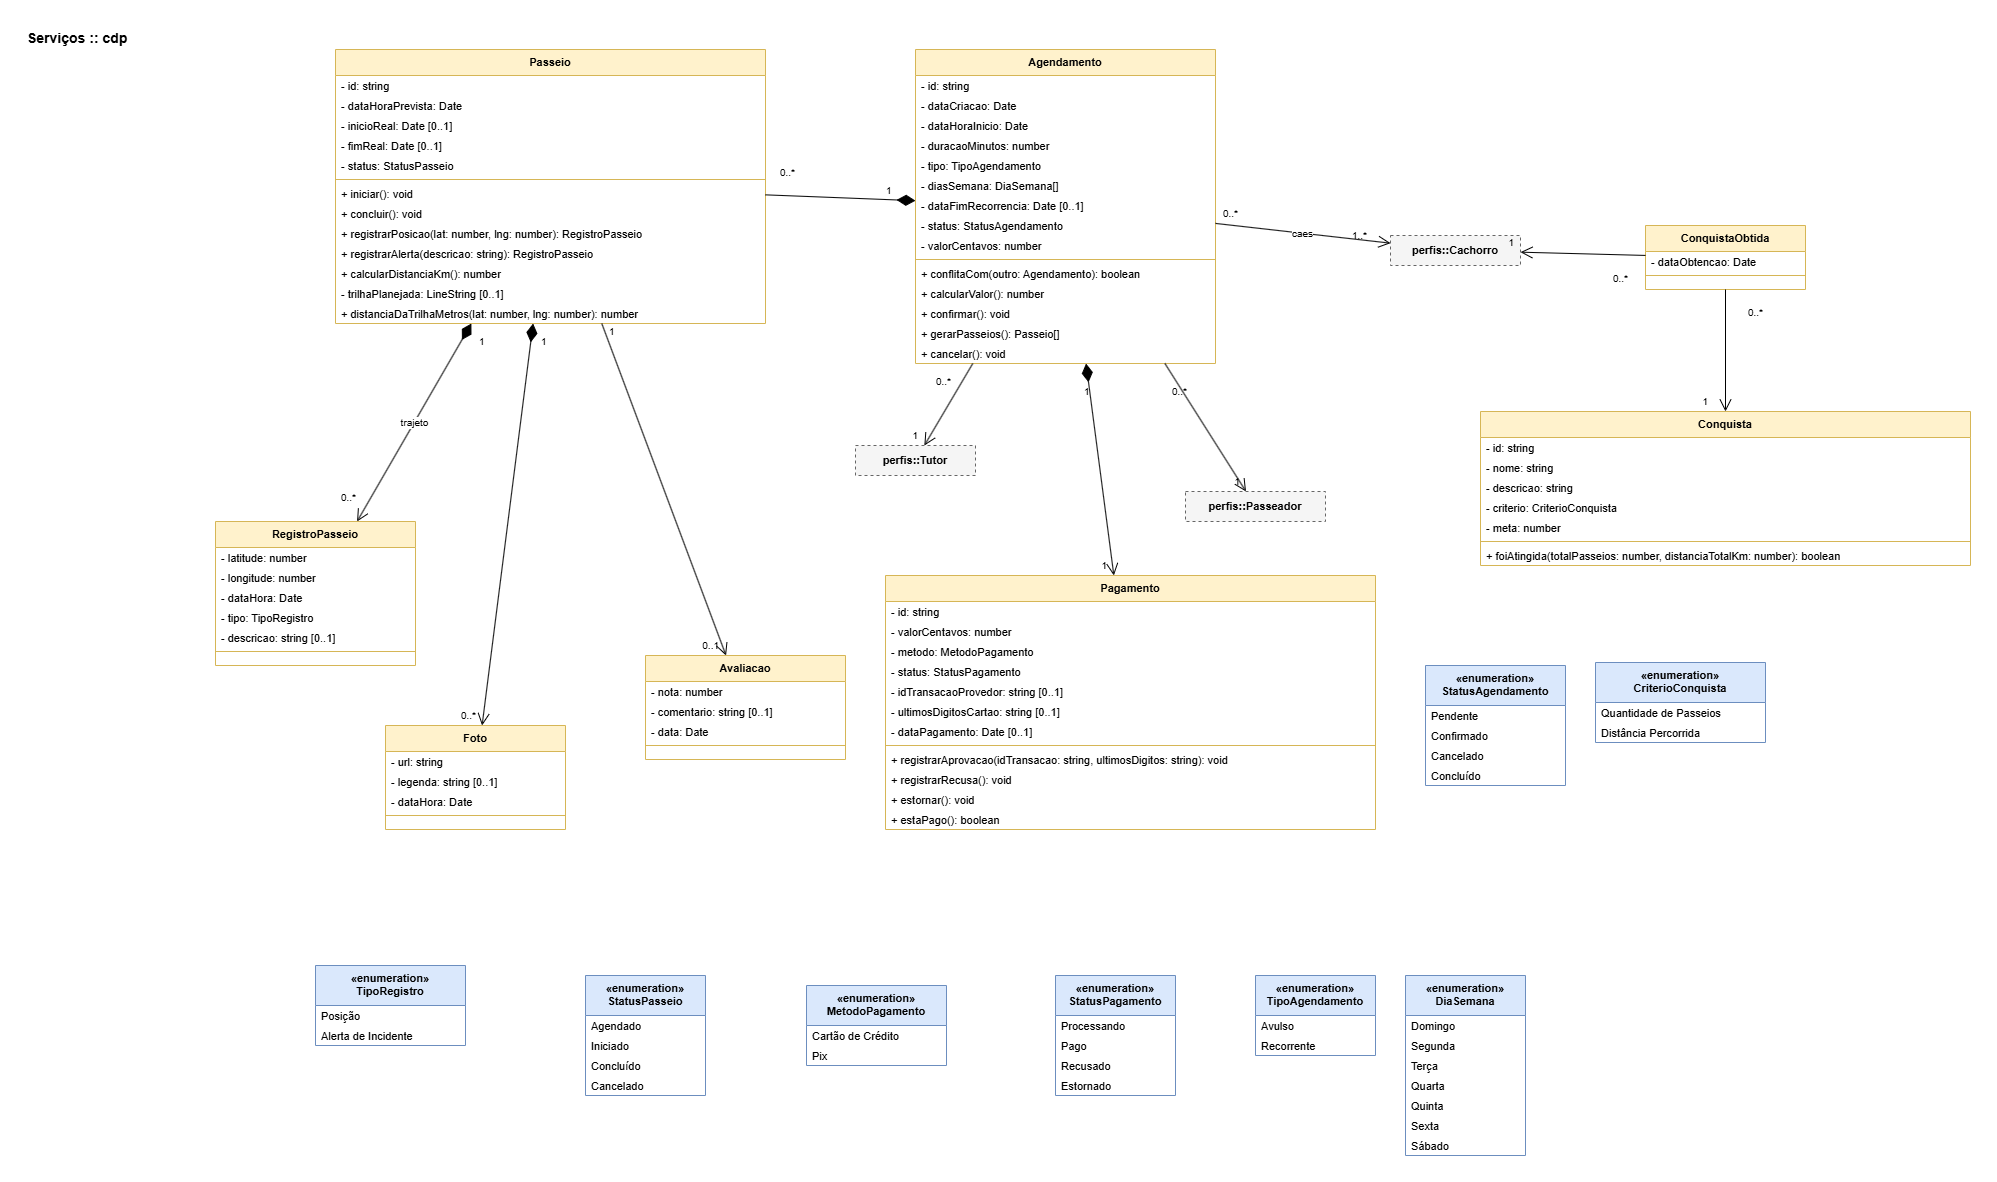
\includegraphics[width=\textwidth]{figuras/ln-servicos-cdp.png}
	\caption{Diagrama de classes do CDP do subsistema Serviços.}
	\label{figura-ln-servicos-cdp}
\end{figure}

As principais classes e métodos são:

\begin{itemize}
	\item \texttt{Agendamento}: tem \texttt{dataCriacao}, \texttt{dataHoraInicio}, \texttt{duracaoMinutos}, \texttt{tipo} (avulso ou fixo), \texttt{diasSemana} e \texttt{dataFimRecorrencia} (só para passeios fixos), \texttt{status} e \texttt{valorCentavos}. Seus métodos são:
	\begin{itemize}
		\item \texttt{conflitaCom(outro)}: indica se dois agendamentos usam o mesmo cão no mesmo horário (RI-5);
		\item \texttt{calcularValor()}: calcula o valor a partir do valor por hora do passeador, da duração e do número de cães;
		\item \texttt{confirmar()}: só muda o status para ``Confirmado'' se o Pagamento estiver ``Pago'' (RI-4);
		\item \texttt{gerarPasseios()}: cria um Passeio para um agendamento avulso, ou um Passeio para cada dia da recorrência de um agendamento fixo;
		\item \texttt{cancelar()}.
	\end{itemize}
	O construtor recusa um \texttt{dataHoraInicio} anterior à \texttt{dataCriacao} (RI-1);

	\item \texttt{Passeio}: tem \texttt{dataHoraPrevista}, \texttt{inicioReal}, \texttt{fimReal} e \texttt{status}. Os métodos \texttt{iniciar()} e \texttt{concluir()} mudam o status e registram o início e o fim reais, conferindo-os com o Agendamento (RI-2 e RI-3). Os métodos \texttt{registrarPosicao(lat, lng)} e \texttt{registrarAlerta(descricao)} só aceitam registros quando o passeio está ``Iniciado''. O método \texttt{calcularDistanciaKm()} soma as distâncias entre as posições do trajeto;

	\item \texttt{RegistroPasseio}: cada ponto do trajeto ou alerta de incidente, com \texttt{latitude}, \texttt{longitude}, \texttt{dataHora}, \texttt{tipo} e \texttt{descricao}. \texttt{Foto} guarda \texttt{url}, \texttt{legenda} e \texttt{dataHora}. As duas classes são partes do Passeio (composição);

	\item \texttt{Pagamento}: tem \texttt{valorCentavos}, \texttt{metodo}, \texttt{status}, \texttt{idTransacaoProvedor}, \texttt{ultimosDigitosCartao} e \texttt{dataPagamento}. Os métodos \texttt{registrarAprovacao(idTransacao, ultimosDigitos)}, \texttt{registrarRecusa()}, \texttt{estornar()} e \texttt{estaPago()} controlam o seu status. O número completo do cartão nunca chega a essa classe;

	\item \texttt{Avaliacao}: \texttt{nota} (de 1 a 5), \texttt{comentario} e \texttt{data}, ligada a um Passeio concluído;

	\item \texttt{Conquista} e \texttt{ConquistaObtida}: \texttt{Conquista} define o critério e a meta (por exemplo, 10 passeios ou 50 km percorridos) e tem o método \texttt{foiAtingida(totalPasseios, distanciaTotalKm)}. \texttt{ConquistaObtida} registra quando um Cachorro recebeu uma Conquista (US13).
\end{itemize}

A regra do limite de cães do passeador (RI-6) depende de todos os agendamentos do passeador naquele horário. Por isso, ela é verificada pela classe de aplicação \texttt{AplAgendamento}, que soma os cães dos agendamentos existentes com os do novo agendamento e compara com o \texttt{limiteCaes} do \texttt{Passeador}.


\subsection{Componente de Gerência de Tarefas}
\label{sec-logica-servicos-cgt}

A Figura~\ref{figura-ln-servicos-cgt} mostra as classes do CGT do subsistema e a Tabela~\ref{tabela-cgt-servicos} descreve suas operações. As classes \texttt{AplPagamento} e \texttt{AplExecucaoPasseio} usam duas interfaces para serviços externos: \texttt{GatewayPagamento}, que envia o pagamento ao provedor externo, e \texttt{NotificadorTempoReal}, que publica as posições e os alertas para o tutor por \textit{Server-Sent Events} (SSE), conforme o RNF-3 (Seção~\ref{rnf-tempo-real}).

\begin{figure}[h!]
	\centering
	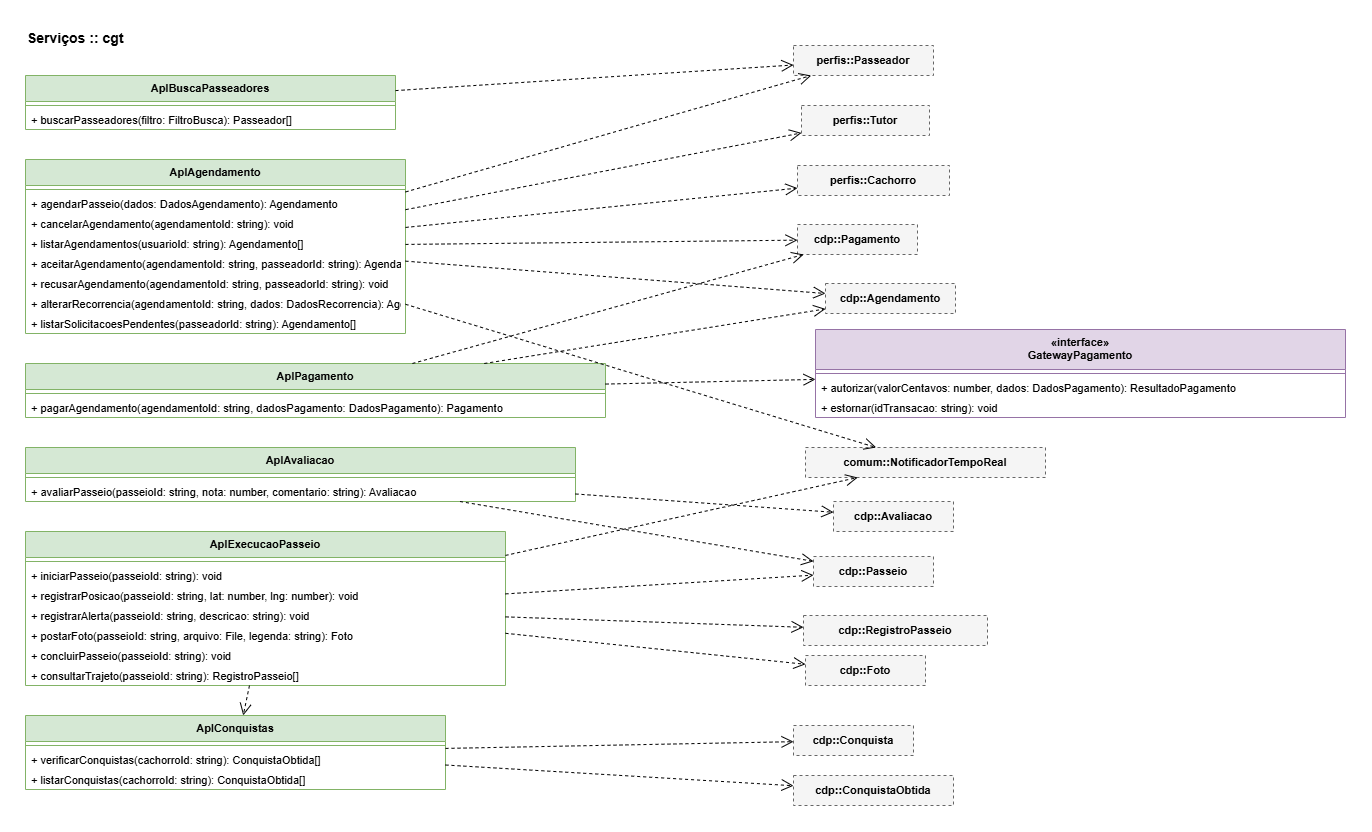
\includegraphics[width=\textwidth]{figuras/ln-servicos-cgt.png}
	\caption{Diagrama de classes do CGT do subsistema Serviços.}
	\label{figura-ln-servicos-cgt}
\end{figure}

\begin{footnotesize}
\begin{longtable}{|p{3.4cm}|p{7.6cm}|p{2.4cm}|}
	\caption{Operações do CGT do subsistema Serviços.}
	\label{tabela-cgt-servicos}\\\hline

	\rowcolor{lightgray}
	\textbf{Classe} & \textbf{Operações} & \textbf{Regras} \\\hline
	\endfirsthead
	\hline
	\rowcolor{lightgray}
	\textbf{Classe} & \textbf{Operações} & \textbf{Regras} \\\hline
	\endhead

	\texttt{AplBuscaPasseadores} & \texttt{buscarPasseadores(filtro)}: retorna os passeadores validados que atendem a localização, a especialidade e o horário informados, ordenados por distância. & --- \\\hline

	\texttt{AplAgendamento} & \texttt{agendarPasseio(dados)}: cria um agendamento avulso ou fixo, com pagamento pendente. \newline
	\texttt{cancelarAgendamento(agendamentoId)}: cancela o agendamento e os passeios futuros. \newline
	\texttt{listarAgendamentos(usuarioId)}: lista os agendamentos do tutor ou do passeador. & RI-1, RI-5, RI-6 \\\hline

	\texttt{AplPagamento} & \texttt{pagarAgendamento(agendamentoId, dadosPagamento)}: envia o pagamento ao provedor externo; se aprovado, confirma o agendamento e gera os passeios. & RI-4 \\\hline

	\texttt{AplExecucaoPasseio} & \texttt{iniciarPasseio(passeioId)}: inicia o passeio. \newline
	\texttt{registrarPosicao(passeioId, lat, lng)}: guarda a posição e a publica para o tutor. \newline
	\texttt{registrarAlerta(passeioId, descricao)}: registra e publica um alerta de incidente. \newline
	\texttt{postarFoto(passeioId, arquivo, legenda)}: guarda uma foto do passeio. \newline
	\texttt{concluirPasseio(passeioId)}: conclui o passeio e chama \texttt{AplConquistas}. \newline
	\texttt{consultarTrajeto(passeioId)}: retorna o trajeto, só para o tutor e o passeador do passeio. & RI-2, RI-3 \\\hline

	\texttt{AplAvaliacao} & \texttt{avaliarPasseio(passeioId, nota, comentario)}: registra a avaliação de um passeio concluído. & --- \\\hline

	\texttt{AplConquistas} & \texttt{verificarConquistas(cachorroId)}: confere o histórico do cão e cria as novas conquistas obtidas. \newline
	\texttt{listarConquistas(cachorroId)}: lista as conquistas do cão. & US13 \\\hline
\end{longtable}
\end{footnotesize}

A Figura~\ref{figura-ln-seq-agendar} mostra o diagrama de sequência da operação \texttt{agendarPasseio}, que é a que envolve mais classes no sistema. A sequência é a seguinte:

\begin{enumerate}
	\item A tela de agendamento chama \texttt{agendarPasseio(dados)} da classe \texttt{AplAgendamento};
	\item \texttt{AplAgendamento} busca o \texttt{Tutor}, o \texttt{Passeador} e os \texttt{Cachorro}s nos repositórios de Gestão de Perfis;
	\item Um novo \texttt{Agendamento} é criado, e o construtor verifica a RI-1;
	\item \texttt{AplAgendamento} busca no \texttt{AgendamentoRepository} os agendamentos pendentes ou confirmados no mesmo horário e, para cada um, chama \texttt{conflitaCom()} do novo agendamento (RI-5);
	\item A soma dos cães desses agendamentos com os do novo agendamento é comparada com o \texttt{limiteCaes} do \texttt{Passeador} (RI-6);
	\item O valor é calculado com \texttt{calcularValor()} e é criado um \texttt{Pagamento} com status ``Pendente'';
	\item O agendamento é salvo e devolvido à tela, que leva o tutor para a tela de pagamento.
\end{enumerate}

\begin{figure}[h!]
	\centering
	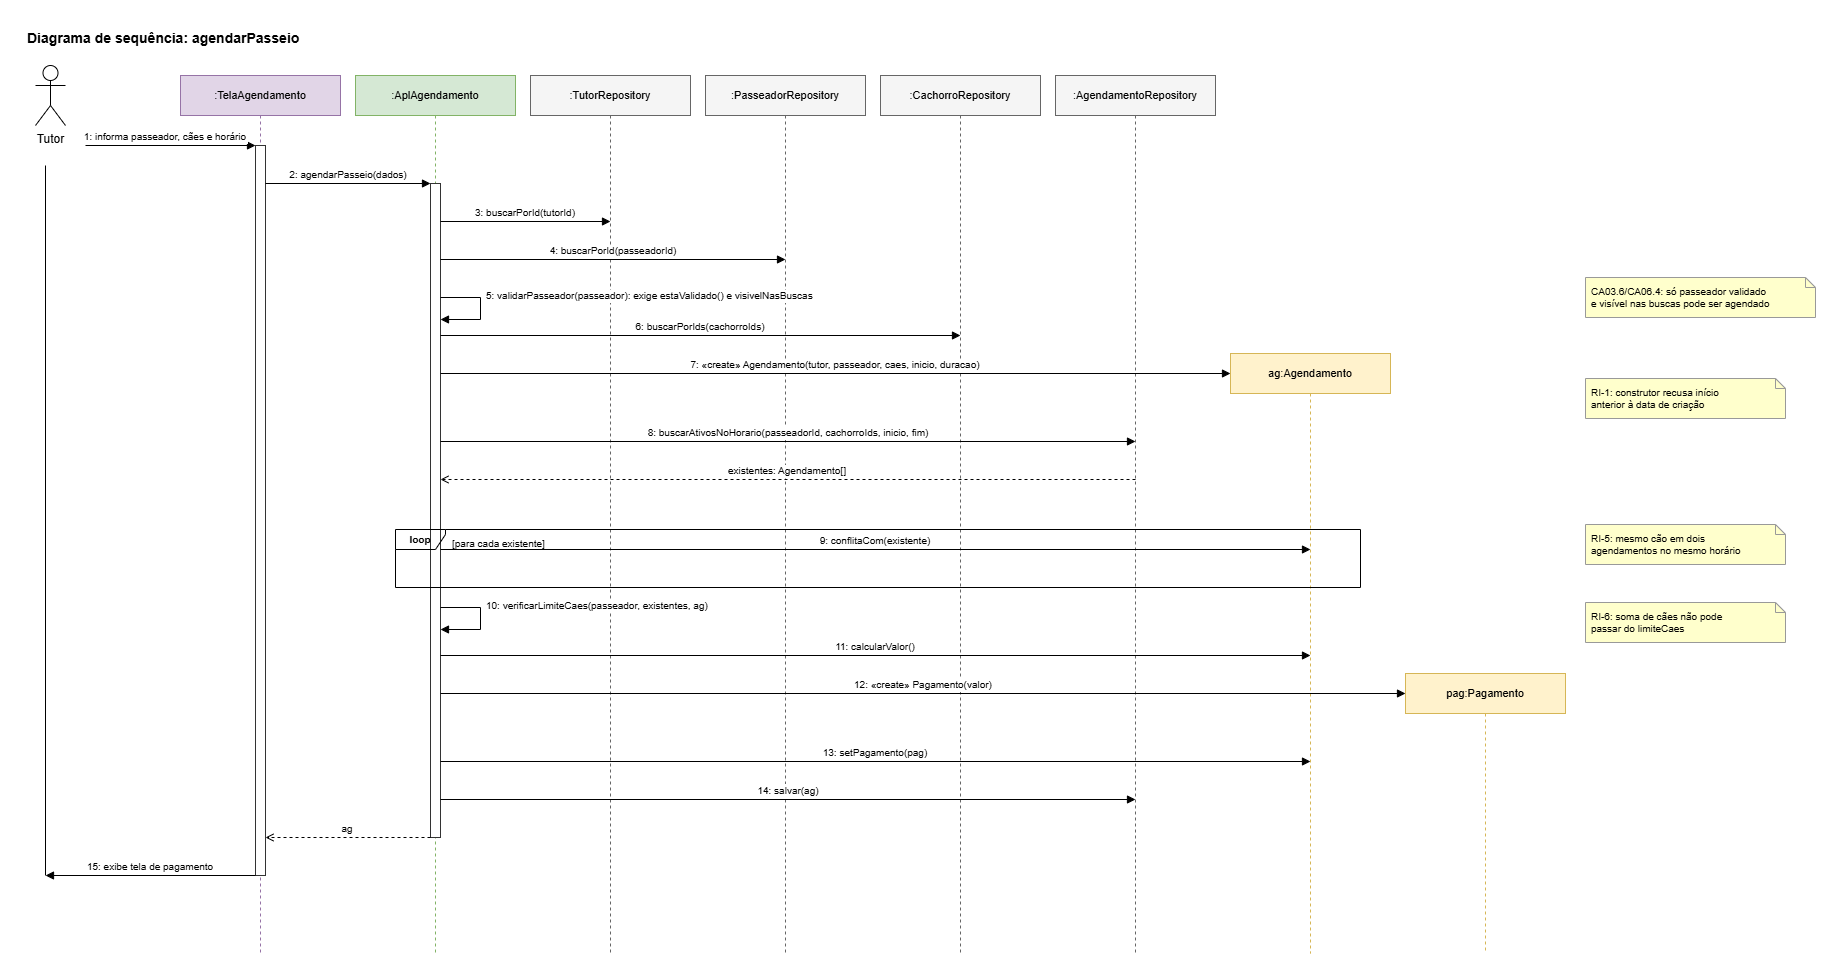
\includegraphics[width=\textwidth]{figuras/ln-servicos-seq-agendar.png}
	\caption{Diagrama de sequência da operação \texttt{agendarPasseio}.}
	\label{figura-ln-seq-agendar}
\end{figure}



\section{Subsistema Suporte}
\label{sec-logica-suporte}

O subsistema Suporte cuida dos chamados abertos por Tutores ou Passeadores e do atendimento feito pelos Atendentes (US16 e US17).


\subsection{Componente de Domínio do Problema}
\label{sec-logica-suporte-cdp}

A Figura~\ref{figura-ln-suporte-cdp} mostra o diagrama de classes do CDP do subsistema Suporte. As classes \texttt{Usuario} e \texttt{Atendente}, de Gestão de Perfis, e \texttt{Passeio}, de Serviços, aparecem no diagrama como classes de outros pacotes.

\begin{figure}[h!]
	\centering
	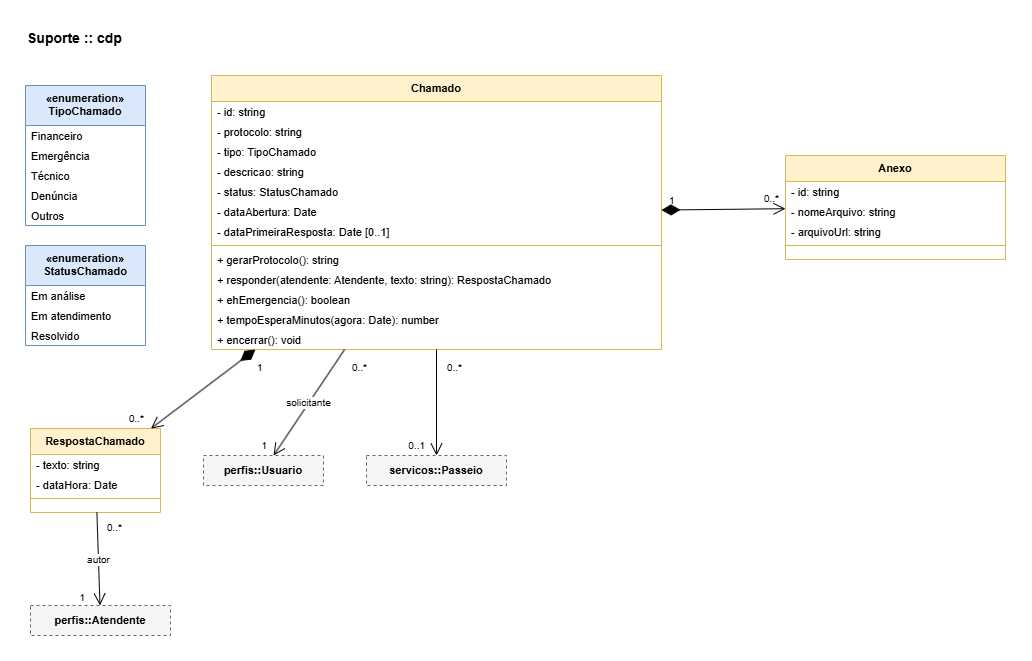
\includegraphics[width=0.85\textwidth]{figuras/ln-suporte-cdp.png}
	\caption{Diagrama de classes do CDP do subsistema Suporte.}
	\label{figura-ln-suporte-cdp}
\end{figure}

As classes deste componente são:

\begin{itemize}
	\item \texttt{Chamado}: tem \texttt{protocolo}, \texttt{tipo}, \texttt{descricao}, \texttt{status}, \texttt{dataAbertura} e \texttt{dataPrimeiraResposta}. Está ligado ao \texttt{Usuario} que o abriu e, opcionalmente, a um \texttt{Passeio}. Seus métodos são:
	\begin{itemize}
		\item \texttt{gerarProtocolo()}: chamado no construtor, que também coloca o status inicial como ``Em análise'' e exige o tipo e a descrição;
		\item \texttt{responder(atendente, texto)}: cria uma \texttt{RespostaChamado}, muda o status para ``Em atendimento'' e, se for a primeira resposta, guarda a \texttt{dataPrimeiraResposta};
		\item \texttt{ehEmergencia()}: indica se o chamado é do tipo ``Emergência'', usado para ordenar a fila de atendimento;
		\item \texttt{tempoEsperaMinutos(agora)}: calcula há quanto tempo o chamado espera a primeira resposta;
		\item \texttt{encerrar()}: muda o status para ``Resolvido''.
	\end{itemize}

	\item \texttt{RespostaChamado}: cada resposta do Atendente, com \texttt{texto} e \texttt{dataHora}, ligada ao \texttt{Atendente} que a escreveu. É parte do Chamado (composição) e guarda o horário de cada resposta para controle interno.
\end{itemize}


\subsection{Componente de Gerência de Tarefas}
\label{sec-logica-suporte-cgt}

A Figura~\ref{figura-ln-suporte-cgt} mostra as classes do CGT do subsistema e a Tabela~\ref{tabela-cgt-suporte} descreve suas operações.

\begin{figure}[h!]
	\centering
	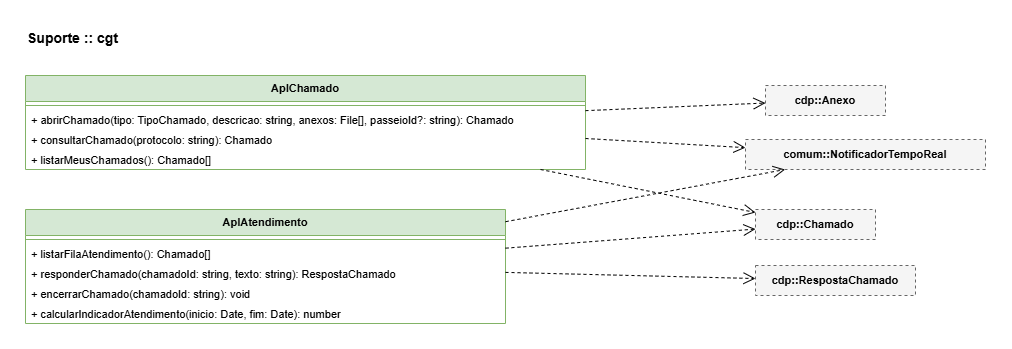
\includegraphics[width=0.85\textwidth]{figuras/ln-suporte-cgt.png}
	\caption{Diagrama de classes do CGT do subsistema Suporte.}
	\label{figura-ln-suporte-cgt}
\end{figure}

\begin{footnotesize}
\begin{longtable}{|p{3.4cm}|p{7.6cm}|p{2.4cm}|}
	\caption{Operações do CGT do subsistema Suporte.}
	\label{tabela-cgt-suporte}\\\hline

	\rowcolor{lightgray}
	\textbf{Classe} & \textbf{Operações} & \textbf{Regras} \\\hline
	\endfirsthead
	\hline
	\rowcolor{lightgray}
	\textbf{Classe} & \textbf{Operações} & \textbf{Regras} \\\hline
	\endhead

	\texttt{AplChamado} & \texttt{abrirChamado(tipo, descricao, passeioId)}: abre um chamado para o usuário autenticado; se for do tipo ``Emergência'', avisa os atendentes pelo \texttt{NotificadorTempoReal}. \newline
	\texttt{consultarChamado(protocolo)}: mostra o chamado e suas respostas. \newline
	\texttt{listarMeusChamados()}: lista os chamados do usuário. & US16 \\\hline

	\texttt{AplAtendimento} & \texttt{listarFilaAtendimento()}: lista os chamados abertos, com os de ``Emergência'' no topo e os demais por ordem de abertura. \newline
	\texttt{responderChamado(chamadoId, texto)}: registra a resposta do atendente. \newline
	\texttt{encerrarChamado(chamadoId)}: encerra o chamado. \newline
	\texttt{calcularIndicadorAtendimento(inicio, fim)}: calcula o percentual de chamados respondidos em até 30 minutos no período. & US17, CA17.2 \\\hline
\end{longtable}
\end{footnotesize}



\section{Requisitos Não Funcionais na Camada de Negócio}
\label{sec-logica-rnfs}

A Tabela~\ref{tabela-rnfs-negocio} mostra como as táticas dos requisitos não funcionais do Capítulo~\ref{sec-rnfs} aparecem no projeto da camada de Negócio.

\begin{footnotesize}
\begin{longtable}{|p{1.6cm}|p{11.8cm}|}
	\caption{Requisitos não funcionais tratados na camada de Negócio.}
	\label{tabela-rnfs-negocio}\\\hline

	\rowcolor{lightgray}
	\textbf{RNF} & \textbf{Elementos da camada de Negócio} \\\hline
	\endfirsthead
	\hline
	\rowcolor{lightgray}
	\textbf{RNF} & \textbf{Elementos da camada de Negócio} \\\hline
	\endhead

	\ref{rnf-multiplataforma} & As regras de negócio ficam apenas no CGT e no CDP, no servidor. O aplicativo móvel e o painel web chamam as mesmas operações, sem repetir regras nos clientes. \\\hline

	\ref{rnf-seguranca-dados} & \texttt{Usuario.senhaHash}; \texttt{Pagamento} guarda só \texttt{idTransacaoProvedor} e \texttt{ultimosDigitosCartao}, e o pagamento é feito pelo \texttt{GatewayPagamento}; \texttt{AplExecucaoPasseio.consultarTrajeto} só devolve o trajeto ao tutor e ao passeador do passeio. \\\hline

	\ref{rnf-tempo-real} & \texttt{AplExecucaoPasseio} publica cada posição e cada alerta pelo \texttt{NotificadorTempoReal} assim que eles são registrados, sem esperar uma nova consulta do tutor. \\\hline

	\ref{rnf-tempo-suporte} & \texttt{Chamado.dataAbertura}, \texttt{Chamado.dataPrimeiraResposta}, \texttt{Chamado.ehEmergencia()} e \texttt{Chamado.tempoEsperaMinutos()}; \texttt{AplAtendimento.listarFilaAtendimento()} ordena a fila e \texttt{calcularIndicadorAtendimento()} mede o critério de aceitação. \\\hline

	\ref{rnf-eficiencia-gps} & \texttt{Passeio.registrarPosicao()} só aceita posições com o passeio ``Iniciado'', o que impede a captura de coordenadas fora do intervalo entre o início e o fim do passeio. \\\hline
\end{longtable}
\end{footnotesize}